%-------------------------------------------------------------
%  INTRODUCTION
%-------------------------------------------------------------

\todo{two sentences introducing Maude}

Maude may be seen as a general framework where to develop model transformations. In this way, some work has been done~\cite{TroyaV10}. Since a term is very general, one could specify graphs or models as terms. Thus, a Maude module can define a \textit{in-place} model transformation, where rewriting rules define transitions between two states or models.

e-Motions~\cite{RiveraDV10} is a Domain-Specific Modeling Language (DSML) and a very general tool that supports the specification and simulation of any real-time DSML. Artifacts developed in e-Motions are translated to Maude in a transparent way. The e-Motions simulation is achieved using the Maude engine. Therefore, e-Motions can be seen as a framework where graphically code in Maude.

\subsection{e-Motions}\label{sub:emotions}
For the sake of comprehension of the rest of the paper, in this section we briefly present e-Motions. The definition of a Domain-Specific Language (DSL) typically comprises three tasks: (i) the definition of its abstract syntax, (ii) the definition of its concrete syntax and (iii) the specification of its behavior.

In e-Motions the abstract syntax is defined by means of a Ecore metamodel, in which all the language concepts and the relations between them are specified. The concrete syntax is provided by defining the so-called Graphical Concrete Syntax (GCS). A GCS is a model (conforms the GCS metamodel) where an image is attached to each concept defined in the abstract syntax.

In e-Motions the behavior of a DSL is specified using visual graph-transformation rules. An e-Motions rule consists of a---possibly conditional---Left-Hand Side (LHS), a Right-Hand Side (RHS) and zero or more Negative Application Conditions (NACs). The LHS defines a (sub)-graph matching, optionally conditional. The RHS specifies a (sub)-graph replacement, which if the rule is applied, every object in the LHS that is not in the RHS is deleted, new objects in the RHS that are not in the LHS are created, and those objects whose attributes (or links) are changed are updated. NACs specify conditions or (sub)-graphs such that if there is a matching, the rule cannot be fired.

Fig.~\ref{fig:assemble} shows an example of an e-Motions rule.\footnote{System documentation and several examples are available at \url{http://atenea.lcc.uma.es/e-Motions}.} The objects in both the RHS and LHS are represented by their images defined in the GCS model. Rule \code{Assemble}'s LHS defines the precondition of the rule. It models a assemble machine who needs both a head and a handle in its connected conveyor. If the \code{NAC1}, stating that the current matched \code{Assemble} has not unfinished other rule, is not satisfied, the rule can be applied. The rule is applied as follows. All objects in the LHS which they do not appear in the RHS are deleted, i.e. \code{he} and \code{ha} objects. Those objects in the RHS which do not appear in the LHS are created, setting their attributes properly, i.e. the \code{ham} object with its three attributes. The rest of objects remain changeless. Moreover, as e-Motions is a framework where to define real-time systems, each rule is applied in a established time, i.e. \code{[prodTime,prodTime]} in the \code{Assemble} rule. A rule may contain zero or more local or auxiliary variables. All attribute or variable assignments and conditions are expressed using Object-Constraint Language (OCL)~\cite{ocl}.

The abstract and concrete syntax, and the behavior of a DSL are models and the e-Motions tool has been developed following MDE principles. The Maude code corresponding to a system defined in e-Motions is generated by an ATL/TCS transformation~\cite{atl}.

\begin{figure}[htp]
  \centering
  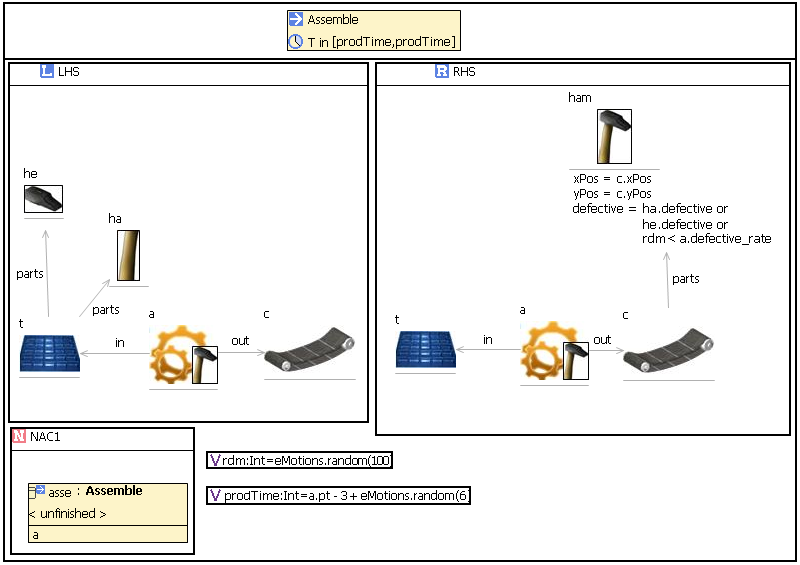
\includegraphics[width=\textwidth]{imgs/assemble}
  \caption{e-Motions \code{Assemble} rule.}\label{fig:assemble}
\end{figure}

